%% Standalone figure for the Statistical Mechanics exercises (Quiz 1).
%% Build: pdflatex quiz1_pt.tex  (or run build.sh in this folder)
\documentclass[11pt,tikz,border=2pt]{standalone}
\usepackage{amsmath,amssymb}
\usetikzlibrary{arrows.meta, positioning}
\begin{document}
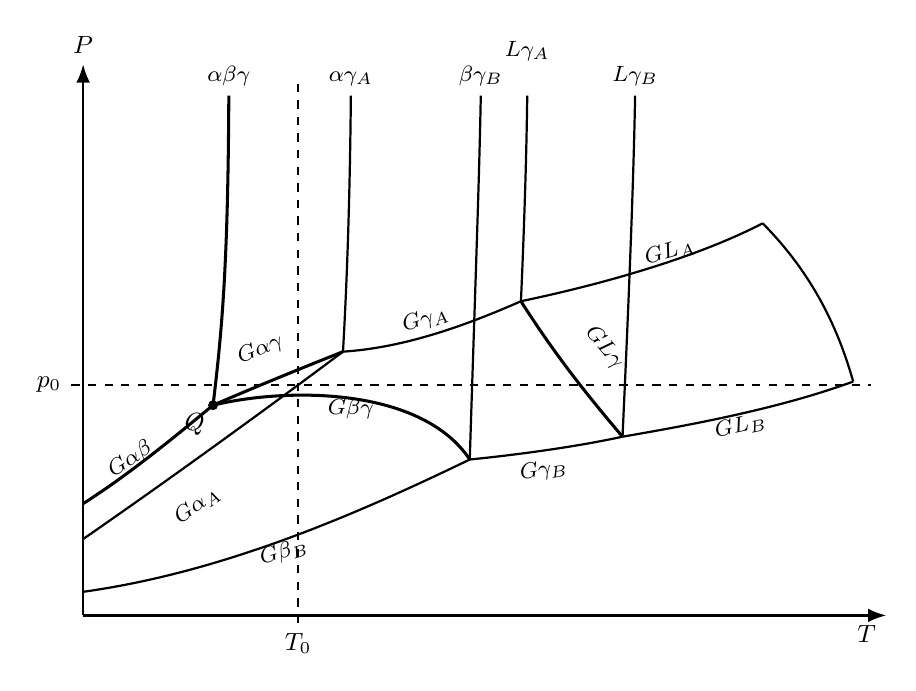
\begin{tikzpicture}[font=\small, >=Latex, line width=0.8pt]
    % axes
    \draw[->] (0,0) -- (10.2,0) node[below left] {$T$};
    \draw[->] (0,0) -- (0,7.0) node[above] {$P$};
    % invariant points
    \coordinate (Q)  at (1.65,2.67);   % quadruple point G alpha beta gamma
    \coordinate (A1) at (3.30,3.35);   % pure A: G alpha gamma
    \coordinate (A2) at (5.56,3.99);   % pure A: G L gamma
    \coordinate (B1) at (4.91,1.98);   % pure B: G beta gamma
    \coordinate (B2) at (6.85,2.27);   % pure B: G L gamma
    \coordinate (CA) at (8.63,4.98);   % critical point of A
    \coordinate (CB) at (9.78,2.97);   % critical point of B
    % binary three-phase curves (thick) and pure-component curves (thin)
    \begin{scope}[line width=1.1pt]
        \draw (Q) .. controls (1.76,3.6) and (1.84,4.4) .. (1.85,6.6);   % alpha beta gamma
        \draw (0,1.42) .. controls (0.6,1.80) and (1.2,2.30) .. (Q);       % G alpha beta
        \draw (Q) .. controls (2.3,2.95) and (2.8,3.15) .. (A1);           % G alpha gamma
        \draw (Q) .. controls (2.6,2.90) and (4.3,2.90) .. (B1);           % G beta gamma
        \draw (A2) .. controls (6.0,3.30) and (6.4,2.80) .. (B2);          % G L gamma
    \end{scope}
    \draw (0,0.97) .. controls (1.2,1.80) and (2.5,2.75) .. (A1);          % G alpha_A
    \draw (A1) .. controls (3.36,4.4) and (3.39,5.5) .. (3.40,6.6);        % alpha gamma_A
    \draw (A1) .. controls (4.1,3.40) and (4.9,3.70) .. (A2);              % G gamma_A
    \draw (A2) .. controls (5.60,4.9) and (5.63,5.8) .. (5.64,6.6);        % L gamma_A
    \draw (A2) .. controls (6.8,4.25) and (7.9,4.60) .. (CA);              % G L_A
    \draw (0,0.30) .. controls (1.8,0.55) and (3.5,1.30) .. (B1);          % G beta_B
    \draw (B1) .. controls (4.98,4.2) and (5.03,5.5) .. (5.05,6.6);        % beta gamma_B
    \draw (B1) .. controls (5.6,2.05) and (6.3,2.15) .. (B2);              % G gamma_B
    \draw (B2) .. controls (6.93,4.0) and (6.99,5.5) .. (7.01,6.6);        % L gamma_B
    \draw (B2) .. controls (7.9,2.45) and (8.9,2.65) .. (CB);              % G L_B
    \draw (CA) .. controls (9.3,4.30) and (9.6,3.60) .. (CB);              % critical locus
    \fill (Q) circle (1.8pt) node[below left=-1pt] {$Q$};
    % isobar p_0 and isotherm T_0
    \draw[dashed, line width=0.6pt] (-0.15,2.93) node[left] {$p_0$} -- (10.0,2.93);
    \draw[dashed, line width=0.6pt] (2.73,-0.1) node[below] {$T_0$} -- (2.73,6.8);
    % curve labels
    \begin{scope}[font=\footnotesize]
        \node[above] at (1.85,6.6) {$\alpha\beta\gamma$};
        \node[above] at (3.40,6.6) {$\alpha\gamma_A$};
        \node[above] at (5.05,6.6) {$\beta\gamma_B$};
        \node[above, yshift=9pt] at (5.64,6.6) {$L\gamma_A$};
        \node[above] at (7.01,6.6) {$L\gamma_B$};
        \node[rotate=33] at (0.60,1.98) {$G\alpha\beta$};
        \node[rotate=35] at (1.45,1.40) {$G\alpha_A$};
        \node[rotate=17] at (2.55,0.80) {$G\beta_B$};
        \node[rotate=22] at (2.25,3.38) {$G\alpha\gamma$};
        \node at (3.40,2.62) {$G\beta\gamma$};
        \node[rotate=17] at (4.35,3.76) {$G\gamma_A$};
        \node[rotate=8] at (5.85,1.84) {$G\gamma_B$};
        \node[rotate=-50] at (6.62,3.40) {$GL\gamma$};
        \node[rotate=16] at (7.45,4.62) {$GL_A$};
        \node[rotate=12] at (8.35,2.40) {$GL_B$};
    \end{scope}
\end{tikzpicture}
\end{document}
